\documentclass[a4paper,
fontsize=11pt,
%headings=small,
oneside,
numbers=noperiodatend,
parskip=half-,
bibliography=totoc,
final
]{scrartcl}

\usepackage{synttree}
\usepackage{graphicx}
\setkeys{Gin}{width=.4\textwidth} %default pics size

\graphicspath{{./plots/}}
\usepackage[ngerman]{babel}
\usepackage[T1]{fontenc}
%\usepackage{amsmath}
\usepackage[utf8x]{inputenc}
\usepackage [hyphens]{url}
\usepackage{booktabs} 
\usepackage[left=2.4cm,right=2.4cm,top=2.3cm,bottom=2cm,includeheadfoot]{geometry}
\usepackage{eurosym}
\usepackage{multirow}
\usepackage[ngerman]{varioref}
\setcapindent{1em}
\renewcommand{\labelitemi}{--}
\usepackage{paralist}
\usepackage{pdfpages}
\usepackage{lscape}
\usepackage{float}
\usepackage{acronym}
\usepackage{eurosym}
\usepackage[babel]{csquotes}
\usepackage{longtable,lscape}
\usepackage{mathpazo}
\usepackage[normalem]{ulem} %emphasize weiterhin kursiv
\usepackage[flushmargin,ragged]{footmisc} % left align footnote

\usepackage{listings}

\urlstyle{same}  % don't use monospace font for urls

\usepackage[fleqn]{amsmath}

%adjust fontsize for part

\usepackage{sectsty}
\partfont{\large}

%Das BibTeX-Zeichen mit \BibTeX setzen:
\def\symbol#1{\char #1\relax}
\def\bsl{{\tt\symbol{'134}}}
\def\BibTeX{{\rm B\kern-.05em{\sc i\kern-.025em b}\kern-.08em
    T\kern-.1667em\lower.7ex\hbox{E}\kern-.125emX}}

\usepackage{fancyhdr}
\fancyhf{}
\pagestyle{fancyplain}
\fancyhead[R]{\thepage}

%meta
%meta

\fancyhead[L]{L. Freyberg, B. Kaden \\ %author
LIBREAS. Library Ideas, 31 (2017). % journal, issue, volume.
\href{http://nbn-resolving.de/
}{}} % urn
\fancyhead[R]{\thepage} %page number
\fancyfoot[L] {\textit{Creative Commons BY 3.0}} %licence
\fancyfoot[R] {\textit{ISSN: 1860-7950}}

\title{\LARGE{Buch, Karow. Ein Ortstermin in zwei Berliner öffentlichen Bibliotheken.}} %title %title
\author{Linda Freyberg \& Ben Kaden} %author

\setcounter{page}{1}

\usepackage[colorlinks, linkcolor=black,citecolor=black, urlcolor=blue,
breaklinks= true]{hyperref}

\date{}
\begin{document}

\maketitle
\thispagestyle{fancyplain} 

%abstracts

%body
\enquote{Wir sind hier ein Brennpunkt.} Sagt Frau Tiepke von der
Stadtteilbibliothek in Berlin Buch. Die Bibliothek ist ein
überschaubarer, durchaus gemütlicher Raum zwischen dem Parkdeck und
einer Fahrschule am Anfang dessen, was nicht wenig euphemistisch
\enquote{Schloßpassage} genannt wird und nicht mehr als eine Ansammlung
gesichtsloser Renditearchitektur der 1990er Jahre ist. In anderer Zeit
hätte man schlicht von einem Nahversorgungszentrum gesprochen. Jeder,
der aus dem Wohngebiet um die Franz-Schmidt-Straße zum Bahnhof Buch
möchte, geht zuerst vorbei am \enquote{Haus der 1000 kleinen Dinge} in
einer ehemaligen Kaufhalle vor der zentral und wie vergessen eine
Bronzeplastik von Gerhard Rommel (Mutter mit Kind, 1980) steht, ihr
gegenüber das Kaufland, dann die Sparkasse und erreicht schließlich über
der Post und nicht zu übersehenen: Die Bibliothek. Das ist ein schöner
räumlicher Pluspunkt: Sie liegt auf dem Weg. Denn zum Bahnhof gehen hier
viele. Die S-Bahn fährt, wenn sie fährt und nicht wegen Signalstörung
auf sich warten lässt, direkt zum Bahnhof Friedrichstraße. In Pankow
kann man aber auch schon umsteigen und die Schönhauser Allee hinunter
ins Herz des Prenzlauer Bergs fahren. Zum Beispiel zur
Bettina-von-Arnim-Bibliothek, deren Raum nicht schöner ist als dieser,
auch gefühlt nicht größer, aber wesentlich überlaufener.

Der Prenzlauer Berg, das ist eine andere Welt, wie auch Frau Tiepke
unterstreicht, aber nicht unbedingt sehnsüchtig. Berlin Buch ist weniger
Bienenkorb. Und es birgt eigene Herausforderungen. Die Idee der
\enquote{Sozialen Bibliotheksarbeit} zum Beispiel ist hier im Prinzip
die Perspektive eines großen Teils der Alltagsarbeit, auch wenn man das
an dem heißen Freitagnachmittag nicht so spürt. Was man auch nicht
direkt spürt, ist das Konfliktpotential in der Nachbarschaft. Jedenfalls
direkt in der Passage, die einfach nur an eine der austauschbaren
Fußgängerzonen in ostdeutschen Kleinstädten erinnert. Aber es steht im
Raum, denn hinter ein paar Zeilen Plattenbauten Richtung Campus und
Grenze zum Land Brandenburg steht seit wenigen Jahren ein
Flüchtlingsheim und erleichtert es manchen Anwohnern, ihre Wut und
Enttäuschung zu kanalisieren. \enquote{Wer anders aussieht, wird schon
einmal offen in der Passage angepöbelt.} Berichtet Frau Triepke. Und
ergänzt, dass es sogar ihr selbst schon passiert ist. Man passt schnell
ins Fremdbild in dieser Gegend, die sich die Bezirkszugehörigkeit mit
einem der linksliberalsten und arriviertesten Wohnviertel der
Bundesrepublik teilt. \enquote{Pankow ist bunt. 18,5 \% der Bewohner
haben ausländische Wurzeln. Die meisten stammen aus Italien, Polen,
Frankreich, den USA und Syrien, wobei die Verteilung je Ortsteil sehr
unterschiedlich ist.} Informiert das Bezirksmagazin Pankow in seiner
aktuellen Ausgabe. Und umschreibt damit denkbar vorsichtig, was man hier
im Stadtbild deutlich sieht: Wer mit ausländischen Wurzeln in
Berlin-Buch wohnt, tut dies vor allem im Rahmen der
Flüchtlingsunterbringung. Wohlhabende EU-Ausländer und die globale
Hipsterkultur steigen spätestens am Bahnhof Pankow aus der stadtauswärts
fahrenden S-Bahn.

Schade eigentlich. Der Schloßpark von Buch ist nämlich eine kleine
Idylle, nach der man sich am Falkplatz nur sehnen kann. Am Eingang
wartet eine freundliche Sandsteinstele, die Mitwelt heißt und vom
Bildhauer Karl Blümel stammt. Man hört unentwegt Amselgesang in den
Gehölzen am Pankeufer. Auf einer Bank sitzt eine ältere Frau und liest
tatsächlich ein Bibliotheksbuch. Dann allerdings kommt ein
Stimmungsbruch, denn zwei Bänke weiter sitzen drei junge Männer mit
Raspelhaarschnitt in Schwarz und Tarn gekleidet auf der Lehne ihrer
Bank, halten je eine Bierflasche fest, hören harte Musik und rufen den
Vorrübergehenden ein markiges \enquote{DEUTSCHLAND!} zu, auf eine
Reaktion wartend. Als wäre die Zeit 1993 stehen geblieben. Sie sind
jung, sie sind stark. Vielleicht. Kennen sie die Bibliothek? Eigentlich
hätte man sie fragen können.

\begin{figure}
\centering
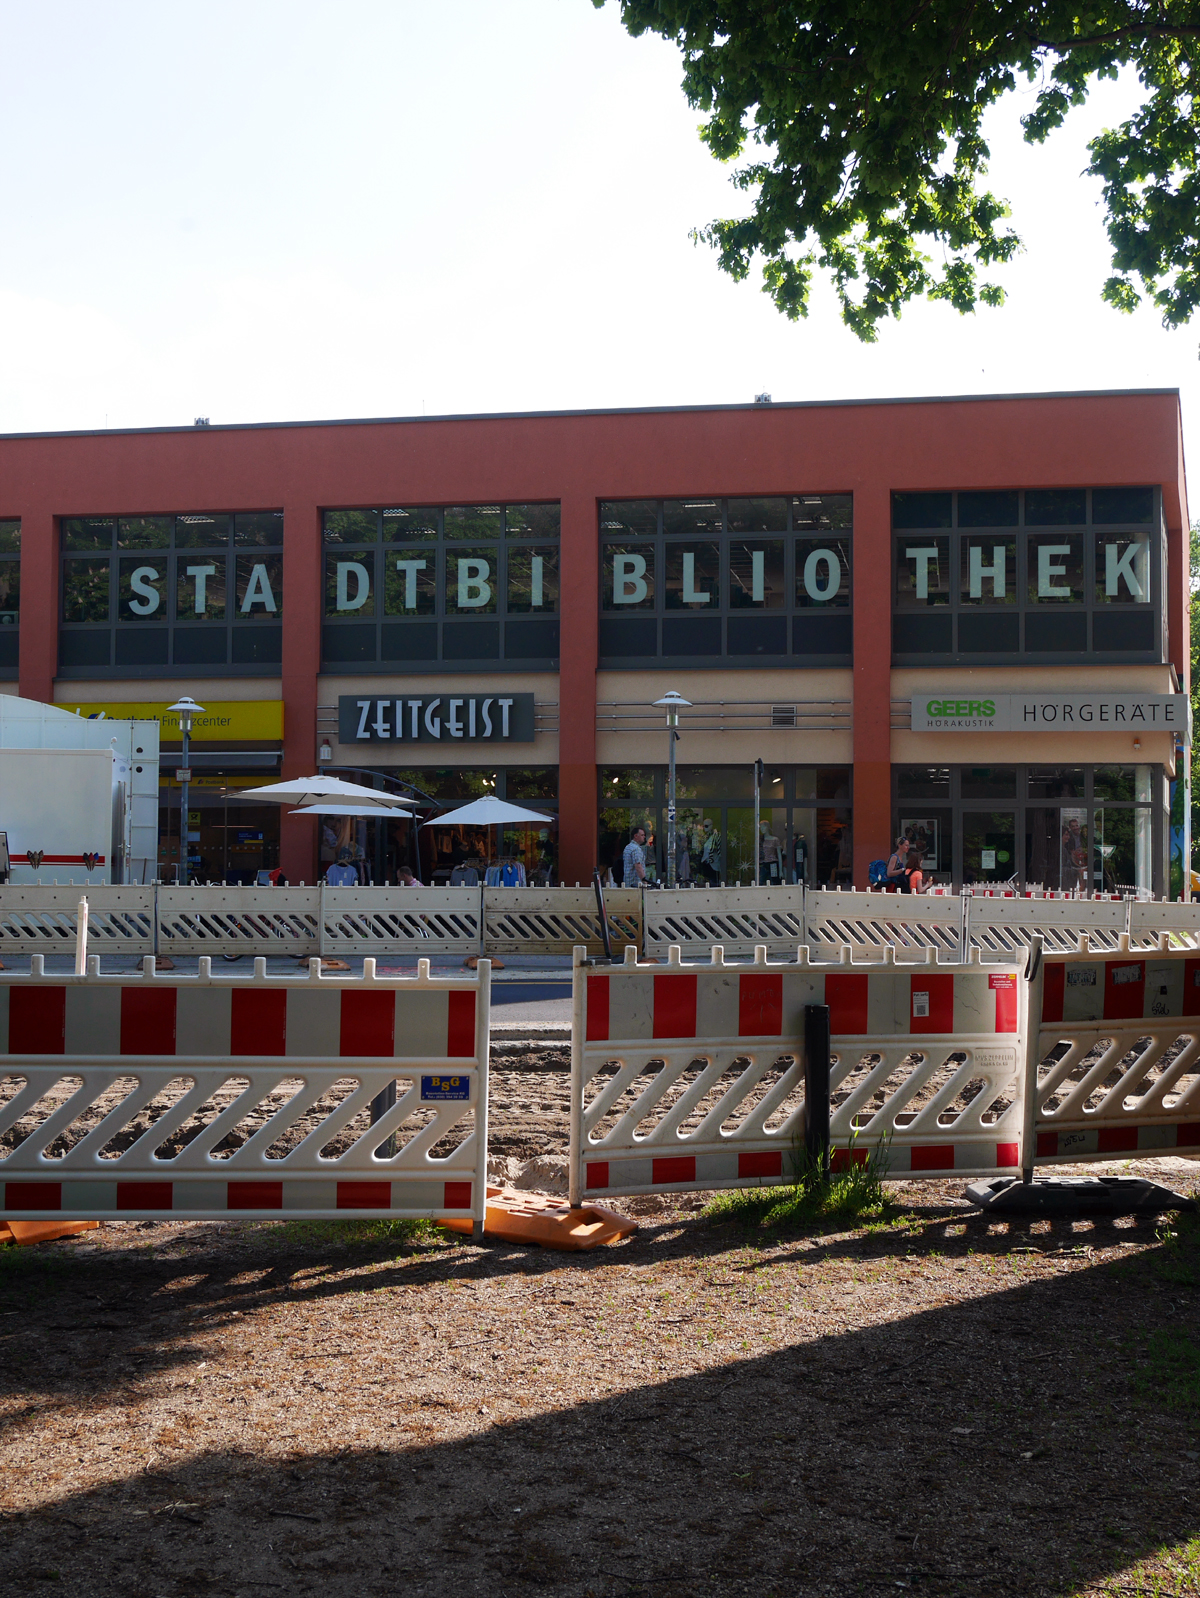
\includegraphics{img/Bibliothek-Buch-1.jpg}
\caption{Die Stadtbibliothek Berlin-Buch}
\end{figure}

\enquote{Wir haben hier in der Tat viele Kinder und Jugendliche, die
nicht in intakten Verhältnissen leben.} Berichtet Frau Tiepke in der
kleinen Kaffeeküche ihrer Bibliothek mit Blick auf den Park. Das prägt
den Bezirk durchaus, auch die Bildungsarbeit, auch die
Bibliotheksarbeit. \enquote{Dazu kommen Leute, die aus den sich
verteuernden Gegenden der Stadt verdrängt werden.} Und jetzt die
Flüchtinge. Sie tut, was sie kann, hat drei Schulklassen am Tag im Haus,
denen sie versucht, die Bibliothek als offenen und sicheren Ort
nahezubringen. Im Winter kam ein Fußballtrainer mit seiner
Jugendmannschaft, weil es zu kalt für Fußball war. Für viele Jugendliche
ist das der Erstkontakt mit der Einrichtung, mit der Idee der
Bibliothek. Frau Triepke freut sich über jeden der wiederkommt. Noch
sind es nicht viele. Sie braucht Zeit. Sie ist erst seit Januar hier.
Sie braucht ein Netzwerk. Sie braucht einen Schlüssel zu dem Kiez ihrer
Bibliothek. Der Bildungsverbund Buch, die lokale Sozialarbeit, das sind
ihre Ansprechpartner. Und das gelingt. Wer sich in solchen Gegenden
engagiert, weiß, dass man allein nicht weit kommt. Bewusst kooperiert
die Bibliothek nun auch mit dem Flüchtlingsheim. Eine Hürde ist, den
dort Wohnenden die Bibliothek überhaupt als Möglichkeit zu vermitteln.
Erwartungsgemäß gelingt dies vor allem über die Arbeit mit Kindern.
Diese haben auch untereinander die wenigsten Berührungsängste. Ab der
fünften Klasse allerdings bleiben sie weg. Die andere zentrale
Nutzer\_innengruppe sind die Senioren. Die kommen oft aus Tradition und
suchen Zerstreuung. Zugleich, wenn auch mitunter implizit, freuen sie
sich über die Bibliothek als stabilen sozialen Anlaufpunkt. Wo man
erkannt und mit Namen angesprochen wird fühlt man sich ein wenig daheim.
Auch hier: Die Bibliothek als offener und sicherer Ort. Dass Frau Tiepke
sich Zeit nimmt und mit ihrer älteren Nutzer\_innen auch mal länger das
Regal durchgeht, um gemeinsam Klappentext für Klappentext auf der Suche
nach einem passenden Buch zu sichten, stärkt dieses Vertrauen. Eine
Buchhandlung gibt es übrigens nicht mehr in Berlin-Buch. Noch ein Grund
für die Bibliothek. Sie versorgt die Menschen. Mit Kontakt und mit
Medien. Das motiviert Frau Triepke. Das fordert sie auch erheblich, denn
die Sparrunden des Bezirkes hinterließen auch hier auf ganzer Linie
Spuren. Der Bestand ist, vorsichtig formuliert, ausbaufähig und
aktualisierbar. Für Veranstaltungen und besondere Programme sind die
Größen Geld, Personal und nicht zu vergessen der Verwaltungsaufwand
alltägliche Hürden. Auf der anderen Seite steht der enorme Bedarf. Man
übernimmt hier, wo eine Bibliothek als Baustein der Bildungsarbeit und
als Anlaufpunkt für viele tatsächlich alternativlos ist, Verantwortung
für die Nachbarschaft und ihre Menschen. Das soziale Klima des
Stadtteils braucht die Bibliothek. Und könnte sicher noch viel mehr
vertragen. Aber bereits die Tatsache, dass sie von Montag bis Freitag
geöffnet ist, ist bereits viel wert.

\begin{figure}
\centering
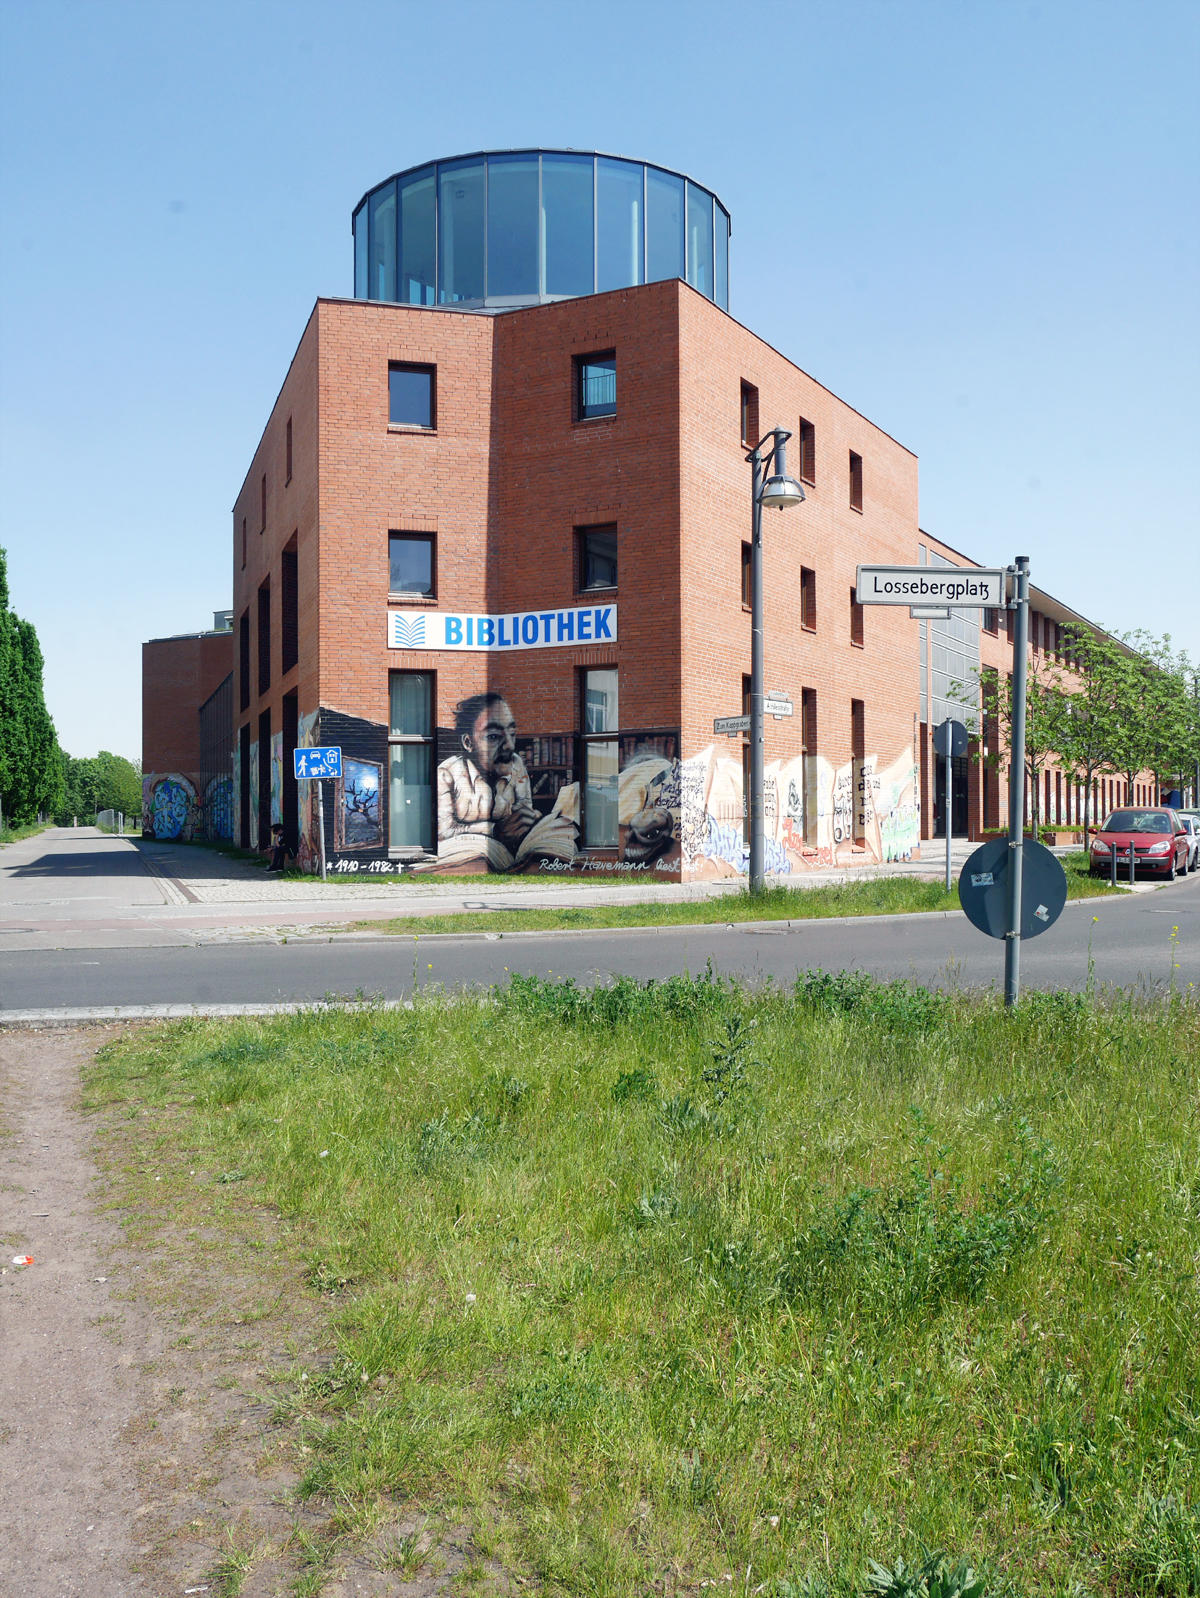
\includegraphics{img/Bibliothek-karow-1.jpg}
\caption{Die Stadtbibliothek Berlin-Karow}
\end{figure}

Dessen wird man sich jedenfalls bewusst, wenn man knapp zwei Kilometer
entfernt und südlich des Berliner Rings die Achillesstraße in Karow
hinuntergeht, zum Robert-Havemann-Gymnasium, in dessen Gebäude die
Stadtplaner dieser etwas künstlichen Neubaunachbarschaft aus den 1990er
Jahren die Stadtteilbibliothek integrierten. Vermutlich stellten sie
sich einen besonders engen Bezug zur Schule vor, deren Pausenklingel die
Bibliothek mitbeschallt. In jedem Fall dürften sie nicht angenommen
haben, dass die Türen sich überhaupt nur an zwei Tagen für die
Nutzer\_innen öffnen. Es fehlt das Personal beziehungsweise eigentlich
natürlich wie immer das Geld, um zusätzliche Mitarbeiter\_innen
einzustellen. Aktuell sind Frau Ketzer und Frau Schmidt nur zu zweit,
was jeden Urlaubstag zur Planungsherausforderung werden lässt. Beide
Öffnungstage lasten sie meist schon mit der Bewältigung des
Leihgeschehens umfassend aus. Denn nachgefragt wird die Bibliothek mit
ihrem deutlich größeren Bestand im Vergleich zu Buch durchaus.

Sie würde sicher auch als Ort sehr gut nachgefragt, stände sie öfter
offen. Denn der Bibliotheksraum ist wirklich schön, hell und luftig mit
breiten Fensterfronten und einer hohen Decke, einen sehr einladenden
Veranstaltungsraum gibt es obendrein. Aber mehr als eine Veranstaltung
im Jahr zu organisieren, ist so gut wie unmöglich. Hajo Schumacher war
neulich da und es war großartig. Berichten Frau Ketzer und Frau Schmidt.
Auch sehr gut besucht. Und man glaubt es gern. Wie Buch ist auch Karow
Teil von Berlin und auch Teil von Pankow. Seine Einwohnerzahl ist sogar
größer als die von Buch. Aber wirklich urban ist der Stadtteil mit
Geschäften die \enquote{Kerstins versunkene Modewelt} und
\enquote{Hundepflege Schnauzbart} heißen, nicht. Ist Buch vom
industriellen Wohnungsbau der DDR geprägt, sind es hier
Einfamilienhäuser. Karow wirkt wie eine brandenburgische Kleinstadt,
sehr suburban. Dass das Neu-Karow genannte Quartier um die
Achillesstraße auch zahlreiche Fünfgeschosser aufweist, ändert daran
wenig. Es wirkt wie ein Ort auf der grünen Wiese und ist das ja
genaugenommen auch. Was man hier tut, wenn man jung ist, lässt sich
nicht so leicht ermitteln. Drei Teenager sitzen zwar im Schatten der
Bibliothek an diesem sommerlichen Freitagnachmittag, aber sie würden
wohl auch nicht hineingehen, wenn diese geöffnet hätte. Die Jugendlichen
sind auch hier nicht wirklich für die Bibliotheksnutzung zu begeistern.
Kinder dagegen kommen in großer Zahl. Und Senioren. Eine stabile
Nutzer\_innenmischung für Stadtbibliotheken in dieser Lage und sicher
nicht nur im Nordosten Berlins.

Eine zweite Parallele zur Bucher Bibliothek ist die neue Zielgruppe der
Geflüchteten. Aber mit anderem Vorzeichen. Wo in Buch Ressentiments
schon im Straßenbild erfahrbar werden, bemüht sich die Einwohnerschaft
von Karow sehr engagiert um ein friedliches Miteinander. Aus den
Unterkünften kommen vor allem Kinder, meist in Begleitung der Väter,
fast nie begleitet von Müttern. In der Bibliothek finden sie ein
besonderes Regal mit einem kleinen Grundbestand an mehrsprachigen
Kinderbüchern. Auch ein Persisch-Deutsches-Wörterbuch liegt bereit. Ein
Arabisch-Deutsches wäre natürlich auch gut. Welches die Väter oft mehr
benötigten als ihre Kinder. Wie bei anderen Einwanderergenerationen sind
nämlich die Kinder häufig die eigentlichen Sprach- und wahrscheinlich
auch Integrationsträger ihrer Familien. Sobald sie in der Schule sind,
werden sie bilingual. Für die Bibliotheksarbeit ist das eine wichtige
Erkenntnis und für die Integrationspolitik eine große Chance, die leider
angesichts der angespannten Ressourcenlage bisher bestenfalls punktuell
ergriffen werden kann. Sehr schön sind die Medienkoffer des VOEBB mit
Bildwörterbüchern, Emil und den Detektiven und einem Stadtführer
Berlins. Wenn er, wie in Karow, mit Vermittlung nicht unbedingt durch
Bibliothekar\_innen aber vielleicht durch Sozialarbeiter\_innen in die
Flüchtlingsunterkünfte gelangt, lässt sich mit ihm viel machen. Ihn aber
einfach nur als Selbstversorgung auszugeben, funktioniert eher nicht,
wie Frau Tiepke aus Bucher Erfahrung berichtet. Und insgesamt sind die
schönen Koffer angesichts der Herkulesaufgabe, eine sehr große Anzahl
von Menschen und darunter auch sehr viele Kinder zu versorgen, die
insgesamt mit denkbar minimaler materieller Ausstattung zurecht kommen
müssen, nur der berühmte Tropfen auf den heißen Stein. Auch die
Bibliotheken wurden von der Entwicklung seit 2015 massiv überrascht.
Selbst wo ein Bestand an fremdsprachiger Literatur vorhanden ist, sind
in diesen in den allerseltensten Fällen die Muttersprachen der
Geflüchteten eingeschlossen. Und sogar wenn man Mittel für eine
entsprechende Bestandserweiterung hätte, wäre es schwer, diese
systematisch zu leisten, sind doch weder das Angebot auf dem Markt noch
Kompetenzen zur Beurteilung und Auswahl der Medien vorhanden. Kleine
Bibliotheken könnten darüber fast schon erleichtert sein, denn wie hier
in Karow sind sie schon damit sehr herausgefordert, den generellen
Bestand aktuell und für die Nutzer\_innen relevant zu halten. Die
Pankower Sparrunden rissen jahrelang Lücken und dass es jetzt etwas
besser wird, bedeutet nicht, plötzlich aus dem Vollen schöpfen zu
können. Aber immerhin lässt sich hier und da etwas aufzustocken und
austauschen. Für Frau Schmidt und Frau Ketzer heißt es ohnehin, mit sehr
wenigen Ressourcen einer steigenden Nachfrage zu begegnen, denn wie in
den meisten Ecken Berlins wächst die Bevölkerung auch in Karow. Dazu
kommt auch hier ein Stammpublikum und auch hier sehen die
Mitarbeiterinnen in dieser Tatsache eine große Stärke im Unterschied zu
den Innenstadtbibliotheken mit hohen Durchlauf, aber auch nicht immer
extrem besserer Ausstattung.

Eigentlich besitzt Karow das Potential zur Musterbibliothek. Der
Bibliotheksraum ist beeindruckend weit. Die Regale schaffen eine
Gemütlichkeit, es gibt einen sehr einladenden Kinderbereich und für
Gruppenbeschäftigung den separaten Veranstaltungsraum mit kleiner
Leinwand und großem Sortiment an Gesellschaftsspielen. Es gibt
Arbeitstische und WLAN. Auch ein Computerarbeitsplatz mit Drucker ist
vorhanden und wird gern genutzt. Ein zweiter wäre sicher auch nicht
unwillkommen. Zugleich ist man mitten im Kiez, kennt sein Publikum beim
Namen und Geschmack. Man ist in die lokalen bürgerschaftlichen
Aktivitäten eingebunden. Und man hat, wie auch in Buch, zugleich den
Anschluss per Bus, Bahn und Bibliothekssystem an die Dynamik der
Hauptstadt, jedoch ohne von ihr überschwemmt zu werden.

Und man teilt das große Hoffnungszeichen: Gemeinsam mit Buch und den
anderen Pankower Bibliotheken hat man seit recht kurzer Zeit einen
neuen, sehr aufgeschlossenen Bibliotheksleiter, der eine immerhin acht
Jahre vakante Stelle füllt. Allein die Besetzung an sich wurde als
Signal für kommende bessere Zeiten gewertet. Besser bedeutet hier: Mehr
Ressourcen, aber auch mehr Plan. Leitbilder sollen für alle
Einrichtungen des Bezirkes entwickelt werden. Ideen werden wieder
gehört. Dass der Bezirk so floriert wie die Hauptstadt insgesamt könnte
neben den negativen Auswirkungen der Gentrifizierung auch Positives
bringen. Nämlich eine Finanzlage irgendwo über der schwarzen Null, die
die Bereitschaft erhöht, wieder in Bibliotheken zu investieren. In Buch
sollen demnächst ein paar tausend Eigentumswohnungen entstehen. Zugleich
werden sehr viele der Geflüchteten vermutlich dauerhaft in Berlin
bleiben. Die Bevölkerung wächst und mit ihr auch der Bedarf an sehr
vielschichtigen Bibliotheksangeboten. Wer mit den Mitarbeiterinnen in
Buch und Karow spricht, spürt, dass sie sich sogar darauf freuen. Die
Motivation ist nicht das Problem. Aber sie brauchen auch die Ressourcen,
um dieses Potential wirklich und tiefgreifend entfalten zu können.

(Berlin, Juni 2017)

%autor
\textbf{Ben Kaden} ist Bibliothekswissenschaftler an der
Universitätsbibliothek der Humboldt-Universität zu Berlin und
Mitherausgeber von LIBREAS

\end{document}